\documentclass[25pt, a0paper, landscape]{tikzposter}
\usepackage{etstikzposter}
\usepackage{multirow}
\usetikzlibrary{arrows, decorations.markings, arrows.meta,positioning}
\usepackage{overpic}
\usepackage{multicol}
\usepackage{sansmath}
\usepackage[sfdefault]{FiraSans}
\usepackage{amsmath, amssymb, amsthm, amsfonts}

\renewcommand{\familydefault}{\sfdefault}
\sansmath


\begin{document}
\maketitle

% Node for title, authors, and institute
\node [text=titlefgcolor,
    outer sep=0pt,
    minimum width=\textwidth,
    minimum height=8cm,
    align=center,
    fill=titlebgcolor, inner sep=1mm] at (0,11) {  % Adjust yshift as needed

\begin{minipage}[c][][c]{0.77\linewidth}
    \hspace*{30pt} 
    \fontsize{80}{90}\selectfont \textbf{Multi-person Physics-based Pose Estimation for Combat Sports}\\[12pt]
    \hspace*{30pt} 
    \fontsize{60}{80}\selectfont Hossein Feiz$^{1}$ \quad David Labbé$^{1}$ \quad Sheldon Andrews$^{1}$ \\[6pt]
    \hspace*{30pt} 
    \fontsize{50}{60}\selectfont $^1$École de technologie supérieure, Montréal, Québec, Canada % Adjusted font size
\end{minipage}%
\begin{minipage}[c][][c]{0.23\linewidth}
    \hspace*{-300pt}
    
\includegraphics[height=8cm]{figures/image11.png}%
    \hspace*{-10pt} % Adjust spacing between images
    
\includegraphics[height=7cm]{figures/image6.png}%
    \hspace*{-10pt} % Adjust spacing between images
    
\includegraphics[height=7cm]{figures/image5.png}%
    \hspace*{-10pt} % Adjust spacing between images
    
\includegraphics[height=7cm]{figures/image9.png}
\end{minipage}

};

\begin{columns}
\column{0.5}
\block{Introduction}{
    Motion capture from only RGB cameras in a typical sports scene (e.g., boxing), with the presence of coaches, viewers, and close interactions between athletes, brings many challenges, such as heavy occlusion, background crowding, and fast, complicated movements. To address this problematic, a multi-view configuration was used. Our system only required the visibility of an athlete from two cameras. We also created a pipeline using machine and deep learning techniques that automated the process of creating animations.
}

\block{Pipeline}{

\begin{overpic}[scale=3]{figures/pipeline.pdf}
\put(65,19){\fontsize{40}{16}\selectfont$L_{2D}+L_{3D}+L_{\beta}$}
\put(0,2){\fontsize{7}{16}\selectfont$\mathrm{Y}_1$}
\put(88,19){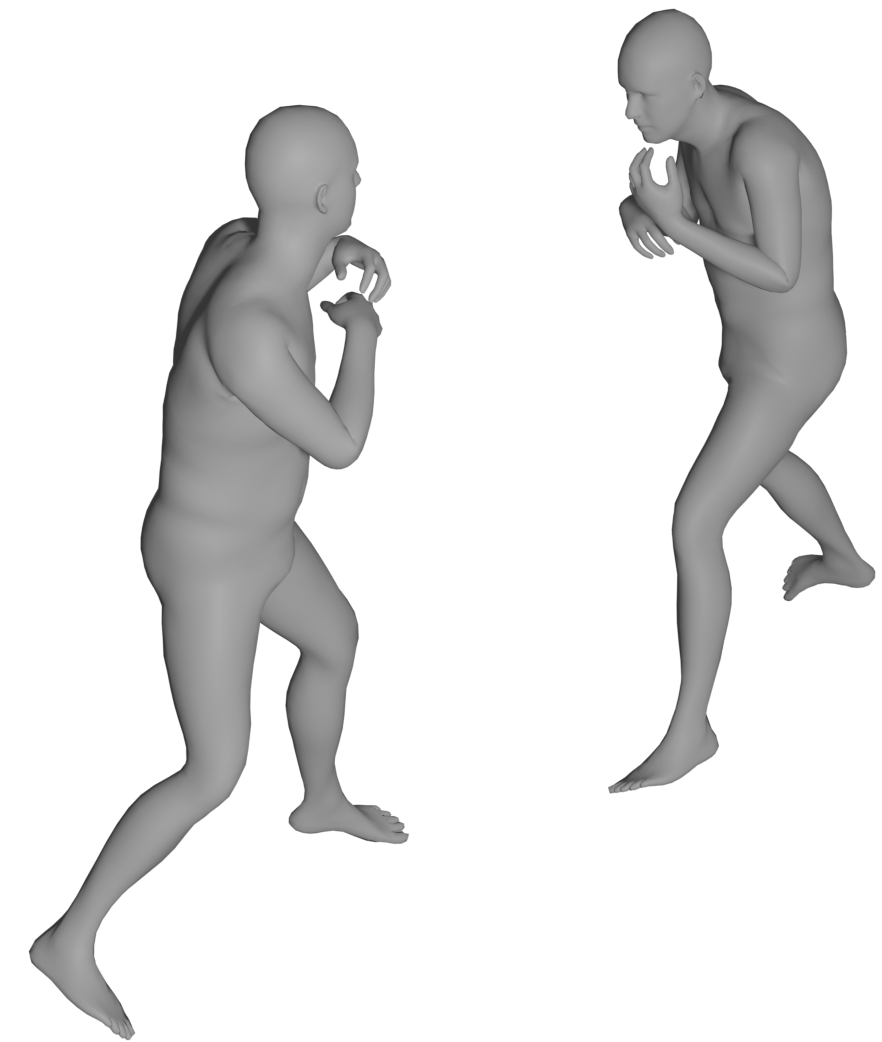
\includegraphics[scale=0.2]{figures/smpl2.png}} 
\put(0.5,8){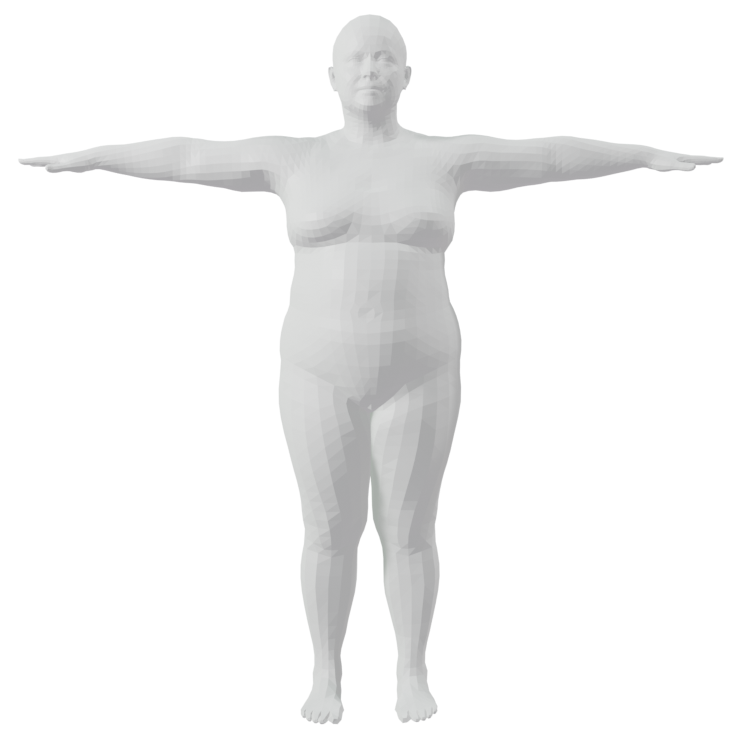
\includegraphics[scale=0.13]{figures/smpl-fat.png}} 
\put(0,0){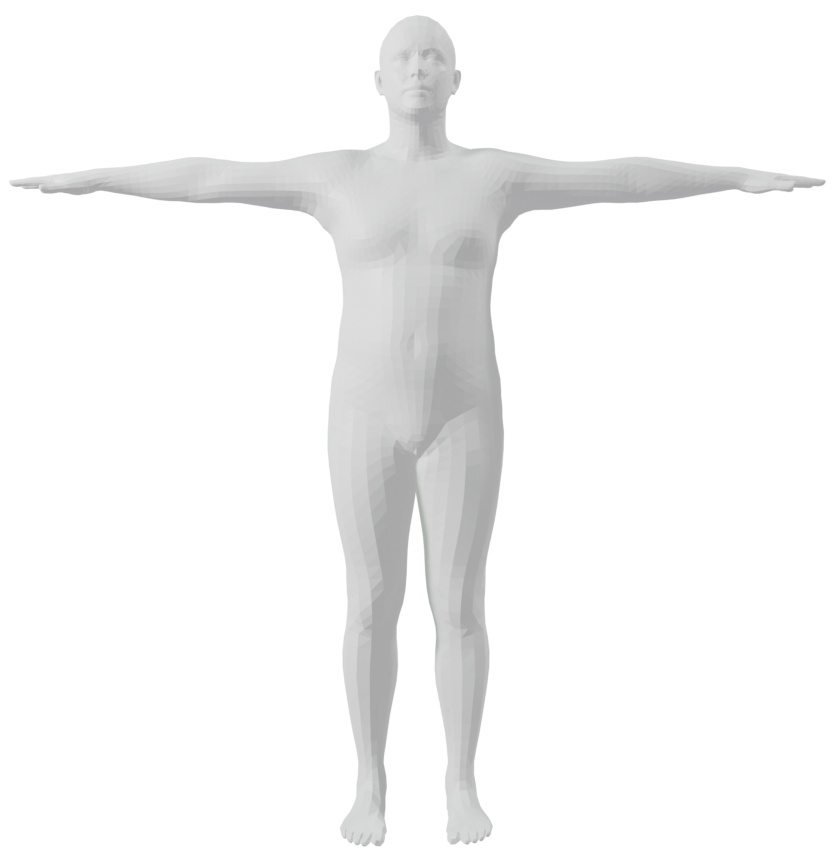
\includegraphics[scale=0.13]{figures/smpl-tall.png}}
\put(88,19){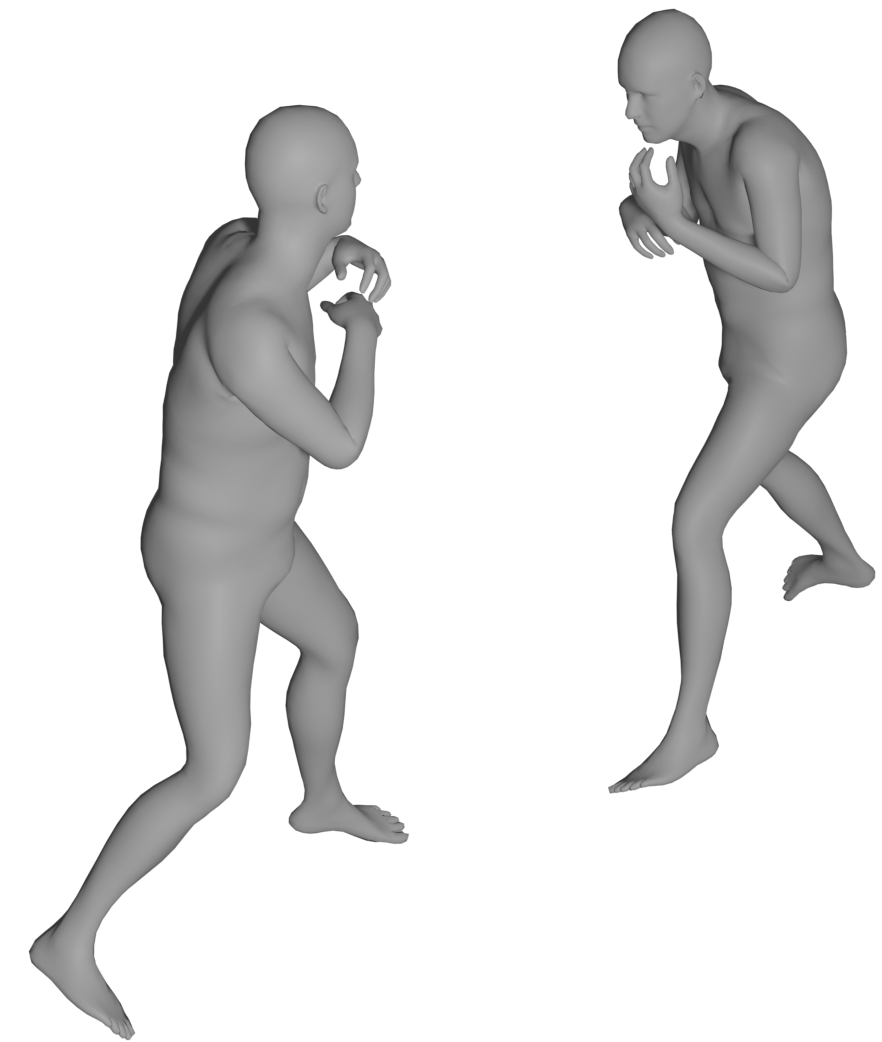
\includegraphics[scale=0.2]{figures/smpl2.png}} 
\put(43.2,8){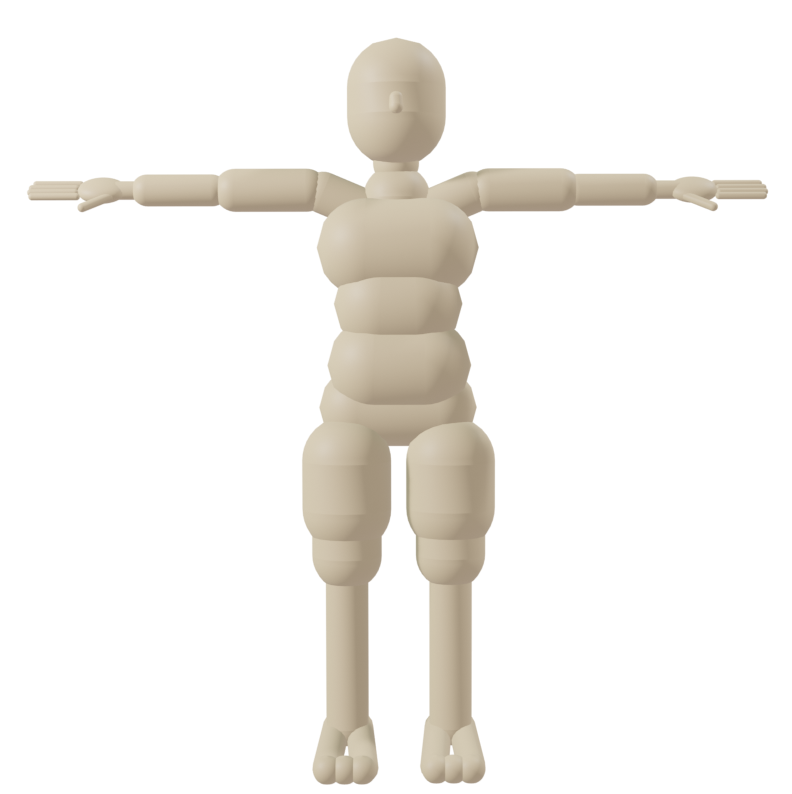
\includegraphics[scale=0.13]{figures/mujoco-fat.png}} 
\put(43,0){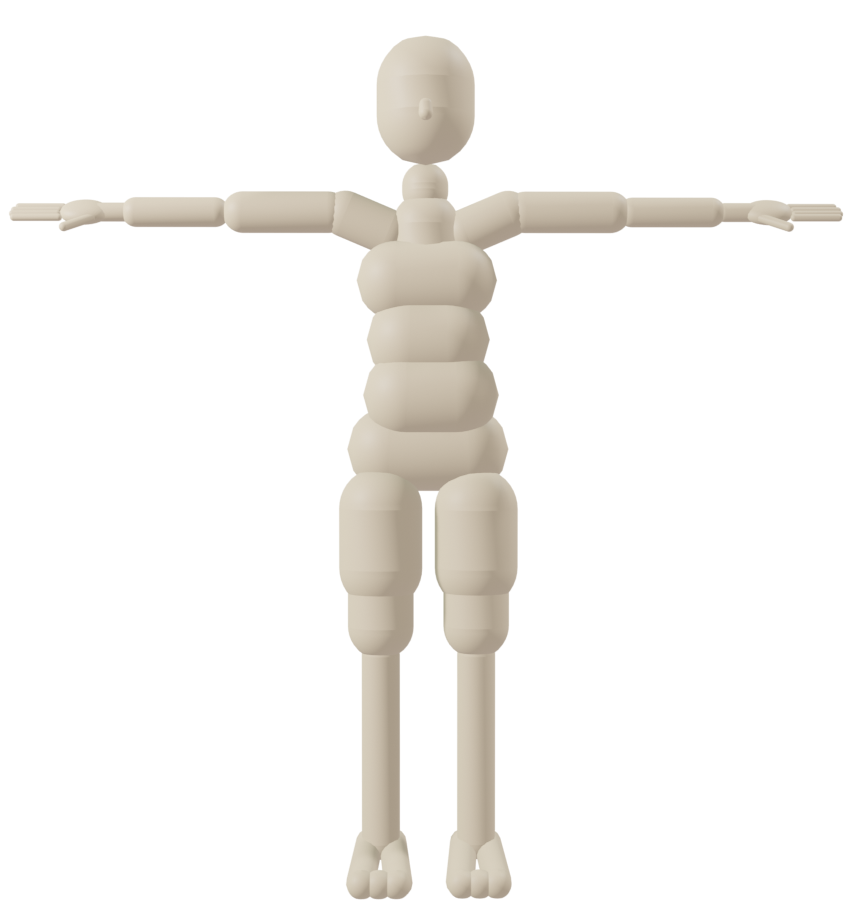
\includegraphics[scale=0.13]{figures/mujoco-tall.png}} 
\put(88,0){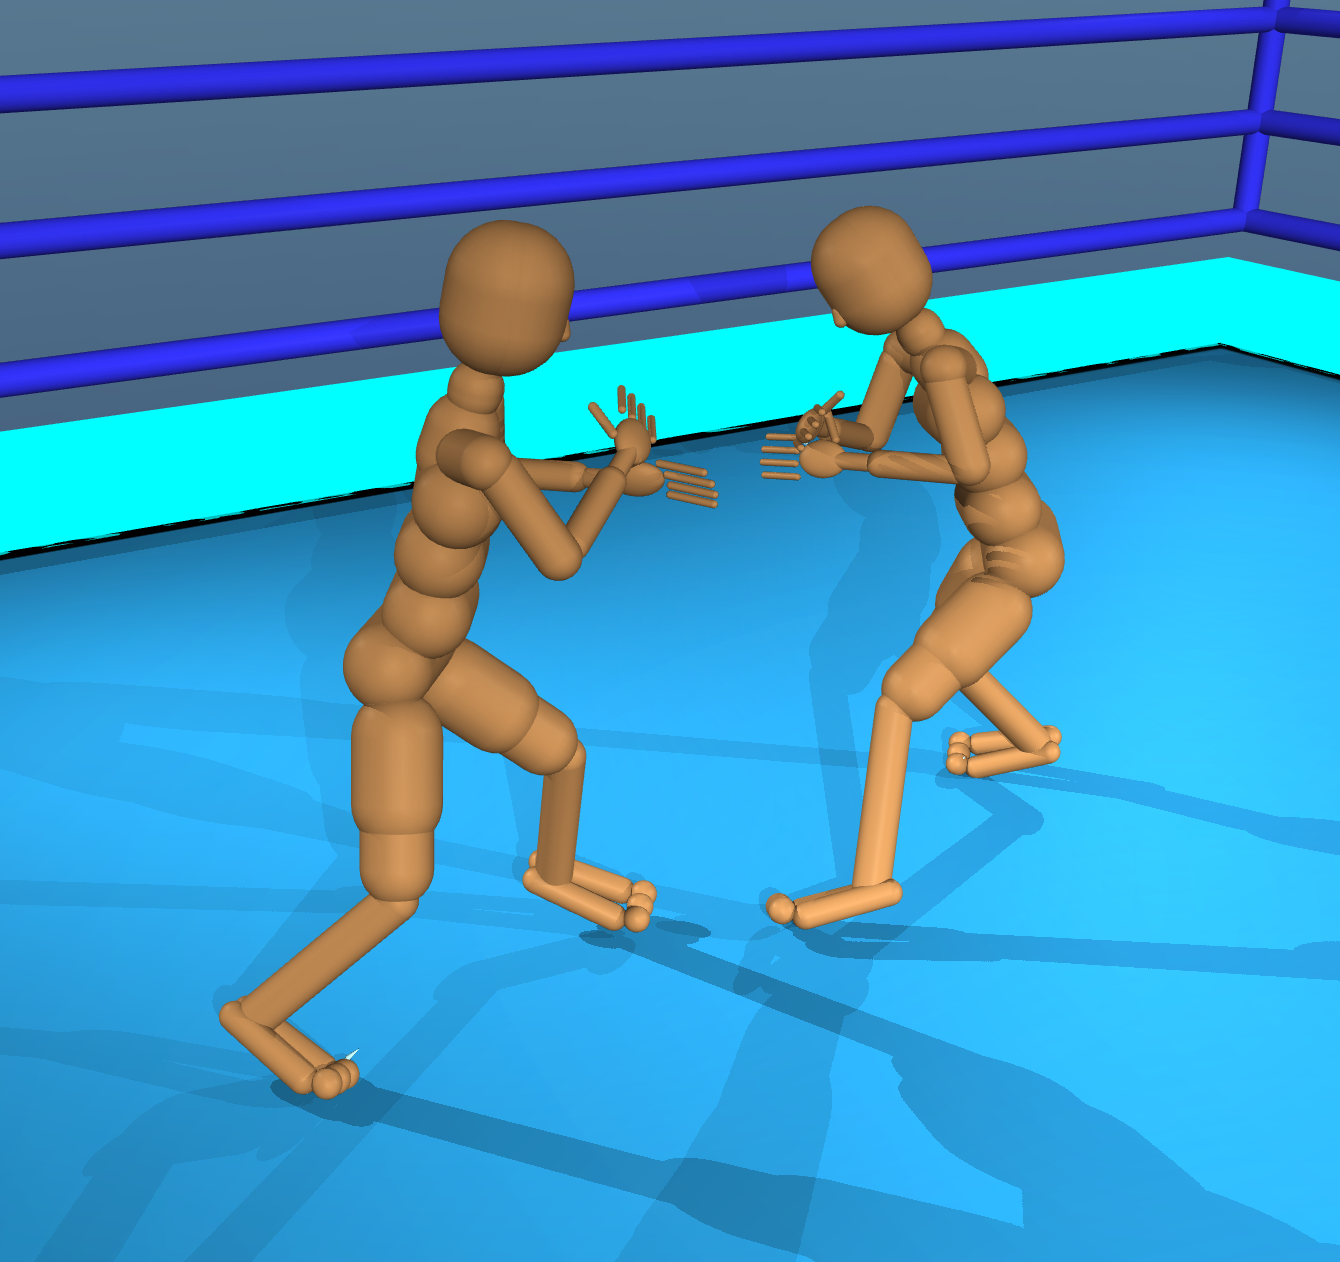
\includegraphics[scale=0.28]{figures/final.png}} 
\end{overpic}}

\block{Multi-frame Multi-view Tracking IDs}{
    \begin{minipage}{0.6\linewidth}
        \begin{itemize}
            \item 1st item on the right
            \item 2nd item on the right
            \item 3rd item on the right
        \end{itemize}
    \end{minipage}
}



\block{Weighted Triangulation and Filtering}{
The weighted triangulation estimates the 3D positions of the keypoints from their corresponding 2D keypoints from all $N$ cameras. The 3D positions of each joint are thus determined by solving the linear system:
\innerblock{Weighted Triangulation}{
\begin{tabular}{p{0.5\linewidth} p{0.45\linewidth}}
\begin{equation}
\begin{bmatrix}
\mu_{1} (\mathbf{P}_{11} - \mathrm{u}_1 \mathbf{P}_{31}) \\
\mu_{1} (\mathbf{P}_{21} - \mathrm{v}_1 \mathbf{P}_{31}) \\
\vdots \\
\mu_{N} (\mathbf{P}_{1N} - \mathrm{u}_N \mathbf{P}_{3N}) \\
\mu_{N} (\mathbf{P}_{2N} - \mathrm{v}_N \mathbf{P}_{3N}) \\
\end{bmatrix}
\begin{bmatrix}
\mathrm{x} \\
\mathrm{y} \\
\mathrm{z} \\
1
\end{bmatrix}
=
\begin{bmatrix}
0\\
\vdots \\
0
\end{bmatrix} \,,
\label{eq:tri}
\end{equation}
&
\begin{minipage}[t]{\linewidth}
$\mathbf{P}_{ij}$ extracts the $i$-th row of the projection matrix $\mathbf{P}_{j}$. $\mu_{j}$ is the average confidence of a 2D point for the current frame in camera $j$. Higher confidence values give more weight to certain cameras. We use SVD to solve Eq.~\ref{eq:tri}.
\end{minipage}
\end{tabular}
}
After triangulation, outliers are handled by interpolating and smoothing using cubic spline for each joint's trajectory. If there is no solution for triangulation, we utilize an extended Kalman filter for dynamic state estimation based on velocity, acceleration of the keypoint, and position constraint to estimate the 3D keypoints. This results in robust filtering and smoothing while preserving trajectory integrity, enabling dependable 3D reconstructions from sparse and noisy 2D keypoints.
}

        
\column{0.5}
\block{Kinematics Optimization}{
Our kinematics optimization refines the SMPL model to minimize the difference between the provided 2D poses ($\mathbf{J}_{\text{2D}}$) from multiple views and 3D keypoints ($\mathbf{J}_{\text{3D}}$) obtained from triangulation. The process ensures temporal coherency and natural motion by incorporating smoothness and human motion priors. An LBFGS optimizer is used to solve the minimization problem, considering various loss terms, including 2D re-projection, 3D alignment, smoothness, and prior losses.

\innerblock{Kinematics Optimization Formulas}{    \begin{align}
      \min_{\theta} \quad & w_1 \, \mathrm{L}_\text{2D} + w_2 \, \mathrm{L}_\text{3D} + w_3 \, \mathrm{L}_\text{reg} +  w_4 \, \mathrm{L}_\text{smooth} + w_5 \, \mathrm{L}_{\text{GMM}} + w_6 \, \mathrm{L}_{\text{Vposer}} \,\,.
    \end{align}
  \begin{multicols}{2}


    \begin{equation}
      \mathrm{L}_\text{2D} = \sum\limits_{\text{j} \in \text{$\mathcal{V}$}} \, \sum\limits_{\text{i} \in \text{$\mathbf{J}_{2D}$}} c_\text{j,i} \rho (\mathrm{J}_{\text{proj}_{j,i}} - \mathrm{J}_{2D_{j,i}})  \,,
    \end{equation}

    \begin{equation}
      \mathrm{L}_\text{3D} = \sum\limits_{i \in \text{$\mathbf{J}_{3D}$}} c_i \| \mathrm{J}_i(\theta, \beta) - \mathrm{J}_{3D,i}\|^2 \,,
    \end{equation}

    \begin{equation}
      \mathrm{L}_{\text{smooth}} = \sum\limits_{t} \| \theta^t - \theta^{t-1} \|^2 + \| \mathcal{M}(\theta^t, \beta) - \mathcal{M}(\theta^{t-1}, \beta) \|^2 \,.
    \end{equation}

    \begin{equation}
    \mathrm{L}_{\text{GMM}} = \frac{1}{N} \sum_{i=1}^{N} \text{GMM}(\theta_i, \beta), \quad \mathrm{L}_{\text{Vposer}} = \frac{1}{N} \sum_{i=1}^{N} (\text{z}(\theta_i)^{2}) \,.
    \end{equation}
  \end{multicols}
}
}

\block{Physics Body Model Generator}{
Since our goal is to reconstruct the motion of $K$ physics-based humanoids at each time step $t$, we define the combined state of all humanoids as $\mathbf{x}_t = (\mathbf{q}_t, \mathbf{v}_t)$, where $\mathbf{q}_t \in \mathbb{R}^{63K}$ and $\mathbf{v}_t \in \mathbb{R}^{62K}$ represent the rotation and velocity of the joints. Whereas $\mathbf{q}_t$ is a minimal coordinate representation of position-level coordinates, we also compute $\mathbf{p}_t \in \mathbb{R}^{21K}$ which are the 3D position of the SMPL joints relative to the humanoid's body frame of reference. This vector is used for the optimization process.  Note that the root orientation is represented as a quaternion. Further details about the humanoid body model can be found in the supplementary material. 
    }
\block{Multi-person Dynamics Optimization}{

The iLQR algorithm optimizes a control trajectory \(\mathbf{u}_{0:T}\) by minimizing the cost function:

\begin{equation}
 \min_{\mathbf{u}_{0:T}} \sum_{t=0}^{T} w_1 \mathrm{L_{\text{reg},t}} + w_2 \mathrm{L}_{\text{p},t} + w_3 \mathrm{L}_{\text{v},t} + w_4 \mathrm{L}_{\text{collision},t} \,.
 \label{eq:mpc_opt}
\end{equation}


The reference positions $\mathbf{p}_{t}$ and velocities $\mathbf{v}_t$ are extracted from the kinematics optimization at each frame $t$, and the trajectory optimization is ``warm started'' using control parameters $\mathbf{u}_{t-1}$ from the previous frame.


The control is updated iteratively as \(\Delta\mathbf{u}_t = \mathbf{K}_t\Delta\mathbf{x}_t + \alpha \mathbf{k}_t\), with \(\mathbf{K}_t\) and \(\mathbf{k}_t\) refined until convergence.
}

\block[titlewidthscale=0.5, bodywidthscale=0.5, titleoffsetx=0cm, bodyoffsetx=0cm, titleoffsetx=-14.5cm, bodyoffsetx=-14.5cm]{Block 1}{
    Content for the first block.
}

\block[titlewidthscale=0.5, bodywidthscale=0.5, titleoffsetx=14.5cm, bodyoffsetx=14.5cm, titleoffsety=6.5cm, bodyoffsety=6.5cm,]{Block 2}{
\begin{figure*}
    \centering
    \scriptsize
    \begin{subfigure}{0.12\linewidth}
        \centering
        \textbf{Frames(Chi3D)} \\[0.2em] 
        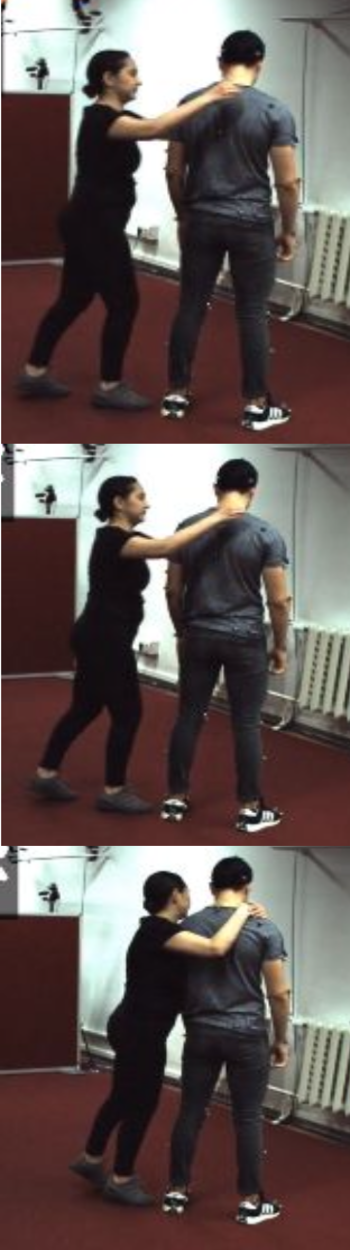
\includegraphics[width=\linewidth, height=6.5cm]{figures/comparison/image5.png}
    \end{subfigure}
    \begin{subfigure}{0.12\linewidth}
        \centering
        \textbf{SLAHMR} \\[0.2em]
        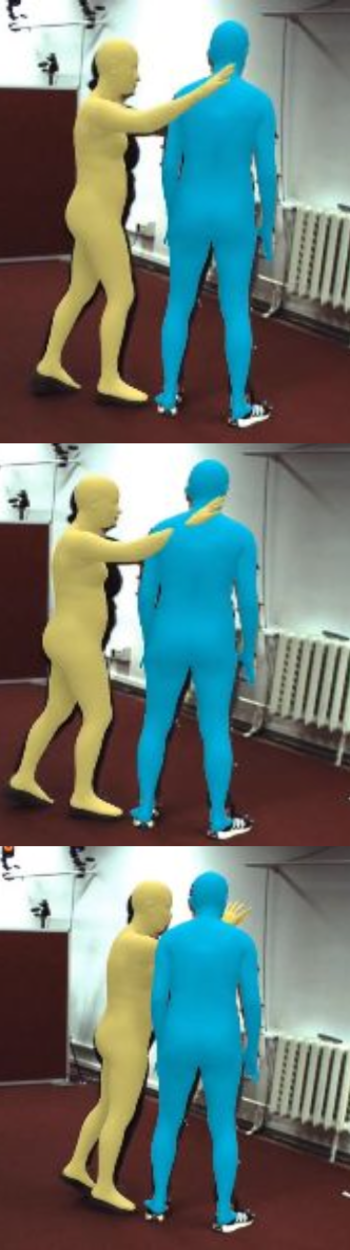
\includegraphics[width=\linewidth, height=6.5cm]{figures/comparison/image6.png}
    \end{subfigure}
    \begin{subfigure}{0.12\linewidth}
        \centering
        \textbf{MultiPhys} \\[0.2em]
        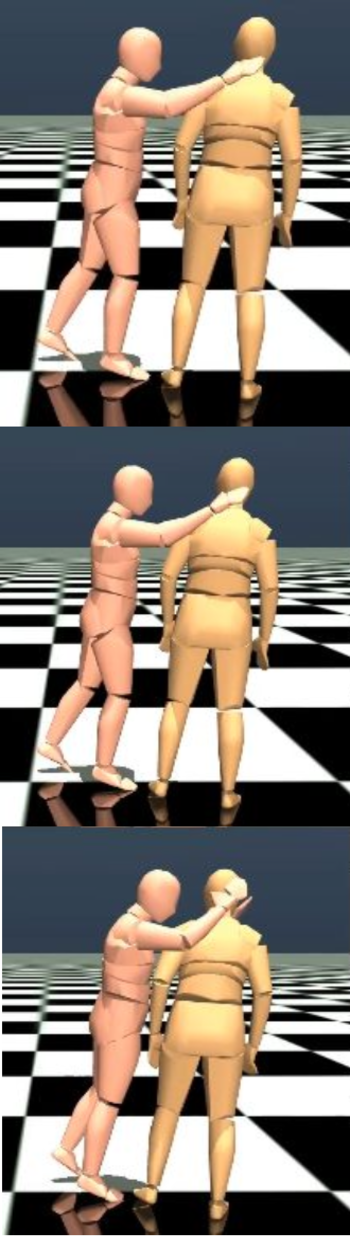
\includegraphics[width=\linewidth, height=6.5cm]{figures/comparison/image7.png}
    \end{subfigure}
    \begin{subfigure}{0.12\linewidth}
        \centering
        \textbf{Ours} \\[0.2em]
        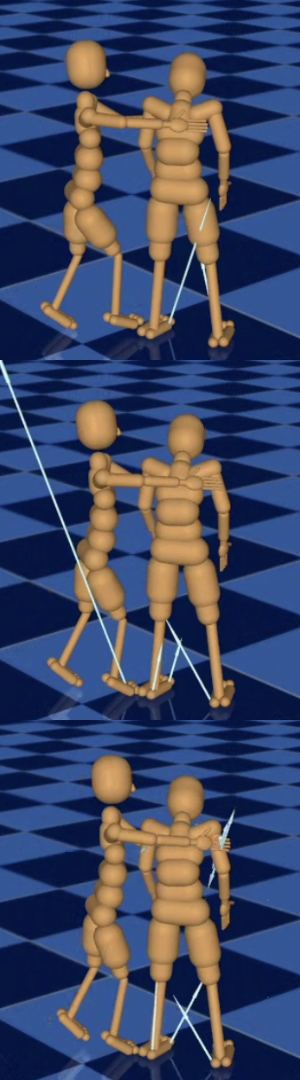
\includegraphics[width=\linewidth, height=6.5cm]{figures/comparison/image8.png}
    \end{subfigure}

\end{figure*}
}

\end{columns}

% Node for images at the bottom of the poster
\node [above right,
    text=titlefgcolor,
    outer sep=0pt,
    minimum width=\textwidth,
    minimum height=2cm,
    align=left,
    fill=titlebgcolor,inner sep=1mm] at (bottomleft) {


};
\end{document}